\documentclass{article}
\usepackage{listings}
\usepackage{amsmath}
%\usepackage{subfigure}
\usepackage{subfig}
\usepackage{amsthm}
\usepackage{amsmath}
\usepackage{amssymb}
\usepackage{graphicx}
\usepackage{mdwlist}
\usepackage[colorlinks=true]{hyperref}
\usepackage{geometry}
\usepackage{titlesec}
\geometry{margin=1in}
\geometry{headheight=2in}
\geometry{top=2in}
\usepackage{palatino}
\usepackage{mathrsfs}
\usepackage{fancyhdr}
\usepackage{paralist}
\usepackage{todonotes}
\setlength{\marginparwidth}{2.15cm}
\usepackage{tikz}
\usetikzlibrary{positioning,shapes,backgrounds}
\usepackage{float} % Place figures where you ACTUALLY want it
\usepackage{comment} % a hack to toggle sections
\usepackage{ifthen}
\usepackage{mdframed}
\usepackage{verbatim}
\usepackage[strings]{underscore}
\usepackage{listings}
\usepackage{bbm}
\rhead{}
\lhead{}

\renewcommand{\baselinestretch}{1.15}

% Shortcuts for commonly used operators
\newcommand{\E}{\mathbb{E}}
\newcommand{\Var}{\operatorname{Var}}
\newcommand{\Cov}{\operatorname{Cov}}
\newcommand{\Bias}{\operatorname{Bias}}
\DeclareMathOperator{\argmin}{arg\,min}
\DeclareMathOperator{\argmax}{arg\,max}

% do not number subsection and below
\setcounter{secnumdepth}{1}

% custom format subsection
\titleformat*{\subsection}{\large\bfseries}

% set up the \question shortcut
\newcounter{question}[section]
\newenvironment{question}[1][]
  {\refstepcounter{question}\par\addvspace{1em}\textbf{Question~\Alph{question}\!
    \ifthenelse{\equal{#1}{}}{}{ [#1 points]}: }}
    {\par\vspace{\baselineskip}}

\newcounter{subquestion}[question]
\newenvironment{subquestion}[1][]
  {\refstepcounter{subquestion}\par\medskip\textbf{\roman{subquestion}.\!
    \ifthenelse{\equal{#1}{}}{}{ [#1 points]:}} }
  {\par\addvspace{\baselineskip}}

\titlespacing\section{0pt}{12pt plus 2pt minus 2pt}{0pt plus 2pt minus 2pt}
\titlespacing\subsection{0pt}{12pt plus 4pt minus 2pt}{0pt plus 2pt minus 2pt}
\titlespacing\subsubsection{0pt}{12pt plus 4pt minus 2pt}{0pt plus 2pt minus 2pt}


\newenvironment{hint}[1][]
  {\begin{em}\textbf{Hint: }}{\end{em}}

\ifshowsolutions
  \newenvironment{solution}[1][]
    {\par\medskip \begin{mdframed}\textbf{Solution~\Alph{question}#1:} \begin{em}}
    {\end{em}\medskip\end{mdframed}\medskip}
  \newenvironment{subsolution}[1][]
    {\par\medskip \begin{mdframed}\textbf{Solution~\Alph{question}#1.\roman{subquestion}:} \begin{em}}
    {\end{em}\medskip\end{mdframed}\medskip}
\else
  \excludecomment{solution}
  \excludecomment{subsolution}
\fi

\newcommand{\boldline}[1]{\underline{\textbf{#1}}}

\chead{%
  {\vbox{%
      \vspace{2mm}
      \large
      Machine Learning \& Data Mining \hfill
      Caltech CS/CNS/EE 155 \hfill \\[1pt]
      Miniproject 1\hfill
      Released January $29^{th}$, 2018 \\
    }
  }
}

\begin{document}
\pagestyle{fancy}

\section{Introduction}
\medskip
\begin{itemize}

    \item \boldline{Group members} \\
    Aw Young Qingzhuo, Ola Kalisz, and Riley Patterson

    \item \boldline{Team name} \\
    Not Hotdog

    \item \boldline{Code} \\
    \url{https://github.com/veniversum/cs155-projects}, see especially the notebooks in \texttt{src}

    \item \boldline{Division of labour} \\
    Qingzhuo implemented the initial structure of the stacked model and many of the initial first-layer models as well, getting early results from submissions to the leaderboard for many of these models. He also accomplished much of the parameter tuning for these models, especially by suggesting randomized CV search rather than grid search.

    Ola worked on parameter tuning for the first layer models for the stacked model. Performed a bunch of grid CV searches based on the results form the randomized CV searches. Analyzed the accuracies for the single models of the initial complex stacked model and together with Riley chose the models to be used in our final two layer stacked model. Retrained some individual models to support the holdout data set.

    Riley worked on addressing overfitting in the stacked model by more selective first-model selection and decreasing the complexity of second-layer models, and by restructuring first model generation to support consistent holdouts. He also wrote a number of scripts to analyze and visualize accuracies of various first-layer models for ease of comparison.

\end{itemize}



\section{Overview}
\medskip
\begin{itemize}

    \item \boldline{Models and techniques tried}

        Our final approach was to stack the results of a wide variety of ``first layer'' models to train a ``second layer'' ensemble model.

        A linear combination of the output of the second layer models are used as our final predictions.

        A huge variety of both linear and non-linear models ranging from nearest neighbor to factorization machines\cite{juan2016field} are used in the first layer in hopes that they will create a dense embedding of the input features. Most of the output of the first layer is the probability of class 1, and a small fraction of them is a binary classification.

        Second layer models are more robust models with good predictive power, and in our case we used AdaBoost with Extra Trees, XGBoost and Neural Nets, all of which are trained with bagging (100-500 bags).

        The first layer models are trained with a 5-fold CV plus holdout, which is reserved for validation of 2nd layer to prevent optimistic bias in validation loss due to data contamination. This is due to the prediction of the $k^{th}$ fold being dependent of the other folds, thus the outputs of the first layer in each fold are not mutually independent of the other fold.

        For parameter search, we instantiated it with using randomized search with cross validation as it is more efficient than grid search \cite{bergstra2012random}. Based on the results of randomized search, for some models, we followed it by grid search to find the best-performing parameters.

        The advantage of the stacked model is that it can outperform each of the individual models due its smoothing nature and ability to highlight each base model where it performs best and discredit each base model where it performs poorly. Stacking is most effective when the base models are significantly different. For this reason, we decided to train a multiple different classifiers as components of the stacked model \cite{gunes2017stacking}.

        For \textbf{first layer models}, we experimented with each of the following, only a subset of which we ended up using in our final model.
        \begin{itemize}
            \item K Nearest Neighbors, we tried different $k$ values and different distance metrics, details later.
            \item AdaBoost
            \item Random Forest
            \item Extra Trees
            \item XGBoost
            \item Logistic Regression
            \item FFM
            \item Vowpal-Wabbit
            \item Neural Nets, here we tried incorporating data from other word representations including like word embeddings.
        \end{itemize}

        For \textbf{second layer models}, we experimented with each of the following:
        \begin{itemize}
            \item Neural Net
            \item Logistic Regression
            \item Adaboost with XTrees
            \item XGBoost
        \end{itemize}

    \item \boldline{Work timeline}
    \begin{itemize}
    % Insert text here. Bullet points can be made using '\item'.
    \item \textbf{Jan 30:} Qingzhuo: set up Colab, initial models. Best performing was MLP Dense(500, ReLU, 0.5 dropout) Dense(500, ReLU, 0.5 dropout) got 0.84440. Tried XGBoost.
    \item \textbf{Jan 31:} Qingzhuo: Begin ensembling some initial NN models with using basic soft/hard voting. got 0.85300. Did cleaning of stems into actual words, word2vec
    \item \textbf{Feb 1:} Qingzhuo: Try AdaBoosting neural nets, SELU self normalizing networks, Log Reg, and bringing them into the voting ensemble
    \item \textbf{Feb 2:} Qingzhuo: worked with libSVM and Vowpal Wabbit and libFFM
    \item \textbf{Feb 3:} Qingzhuo: continued with Feb 2 work, looked into latent support measure machines, TPOT
    \item \textbf{Feb 3:} Ola: worked with Adaboost and Random Forest, for the first layer classifiers. For parameters search, used grid search, based on the previous results from the random search.
    \item \textbf{Feb 4-5:} Qingzhuo: Worked on designing stacked ensemble, choosing models for it. Created notebook for generating meta features from adaboost, random forests, extra tree, logistic regression, libffm, vowpal  wabbit, KNN and xgb.
    \item \textbf{Feb 4:} Ola: Continued working with first layer classifiers and parameters tuning, focused on Adaboost as we tried using it in the second layer of the stacked model, as well.
    \item \textbf{Feb 6:} Qingzhuo: Work on 2nd level meta classifiers, including bagged NN, Adaboosted extra trees and XGBoost
    \item \textbf{Feb 6:} Riley: Made a generic single-dimension parameter search script to analyze existing model results and plot in-sample/validation accuracy vs. parameter values to understand the impact of overfitting and consider selecting simpler models with worse validation accuracy.
    \item \textbf{Feb 7:} Qingzhuo: Worked with StackNet to train 3 level stacked model.
    \item \textbf{Feb 7:} Riley: Split the data to maintain a holdout when training the first layer in order to minimize data leakage/overfitting in cross validation on the second layer. Analyzed our best-performing first layer models and retrained them with this holdout.
    \item \textbf{Feb 7:} Ola: Retrained Adaboost, Random Forest and Extra Trees from first layer with kept holdout data. Designed a simpler 2 level stacked model to prevent overfitting that we encountered with 3 level stacked model. Analyzed the performance of the first layer classifiers and, with Riley, chose 8 best performing out of them to use in the simplified model.
    \item \textbf{Feb 8:} Riley: Experimented with simpler 2 level stacked models to minimize overfitting. Trained a neural net with fewer first layer model outputs as input, and tried logistic regression as well.
    \item \textbf{Feb 8:} Ola: Tried implementing a simpler stacked classifier with AdaBoost with Extra Tree in the second layer. Encountered problems with the implementation, failed attempt.
    \end{itemize}

\end{itemize}



\section{Approach}
\medskip
\begin{itemize}

    \item \boldline{Data processing and manipulation}
    \begin{itemize}
    % Insert text here. Bullet points can be made using '\item'.
        \item \textbf{Bag of Words:} Most models relied on the bag-of-words representation provided with no modification before input to our first layer models
        \item \textbf{TF-IDF:} Term frequency - inverse document frequency approach was a data transformation approach that we tried out. The idea for term frequency is that the reviews (documents) are of different lengths and a longer document contains more words than a shorter one, so the importance of words should be scaled somehow (based on the count of the most frequent word in the document for example). The idea for inverse document frequency is that different words have different distributions amongst documents, and words such as `this' which appears more frequently are not as important as less frequently. Together, term frequency and inverse document frequency gives a weighted measure of importance of words in documents that is normalized regard to the length of the document or frequency of particular words in the document. This technique is used often in information retrieval and text classification \cite{tokunaga1994text,robertson2004understanding,salton1988term,ramos2003using}, but we did not notice a significant improvement in classification accuracy with or without TF-IDF.
        \item \textbf{Lemmatization \& vector embedding:} The words given were stemmed \cite{porter1980algorithm}, which leaves us with roots. While it is effective in reducing derivationally related words to stems, it does it in a rather crude way without considering the morphology of the word (i.e. knives -> kniv). This means that it is rather difficult to extract the semantics of the words from the stems alone. An attempt was made to manually convert them back to lemmas. While by itself this conversion might not do much, we can now convert the words into vector embeddings which preserves some of the semantics of the words \cite{bojanowski2016enriching}. A famous example of this is that the vector representations of the words \textbf{king} - \textbf{male} + \textbf{female} would have the closest similarity measure to \textbf{queen}. We used fasttext implementation with pretrained word vectors for our embeddings\cite{bojanowski2016enriching}.
        This is limited however as vector embeddings greatly increased the dimensionality of our dataset, which makes neural nets one of the only feasible models which can ingest this transformed data. We made use of both locally connected layers as well as convolutional layers which have unshared and shared weights respectively to try to lower the dimensionality of the inputs. We used network topologies of wide and deep networks shown in \cite{cheng2016wide} which combines sparse features along with dense embeddings. The wide model is a linear model which can memorize sparse interactions and the deep model is capable of generalizing better to feature combinations unseen in training. Combining the two allows the models to complement each other for a more robust classifier.
        \item \textbf{Second Layer Model Meta-Features:} The first-layer classifiers of our final model are simply fed with the bag-of-words representations as inputs (an exception here is the convolutional neural network, which uses word embeddings). Every first layer classifier returns a vector of class predictions (for some models we used the probability of the class instead) for every data point. The idea for the second layer is to ``stack'' the predictions (or prediction probabilities) from different classifiers together to create a vector of meta features for every data point. Such a feature vector is fed as input to the second layer classifier which outputs the final prediction of the model. (Note that we also tried using 3 layer architecture where we stack predictions from second layer and feed them to third layer which return final prediction.) This idea is well explained in \cite{gunes2017stacking} (although they use a more sophisticated model with bootstrap replications) and can be illustrated by a diagram, see figure \ref{stack}.
        \begin{figure}[H]
        \centering
        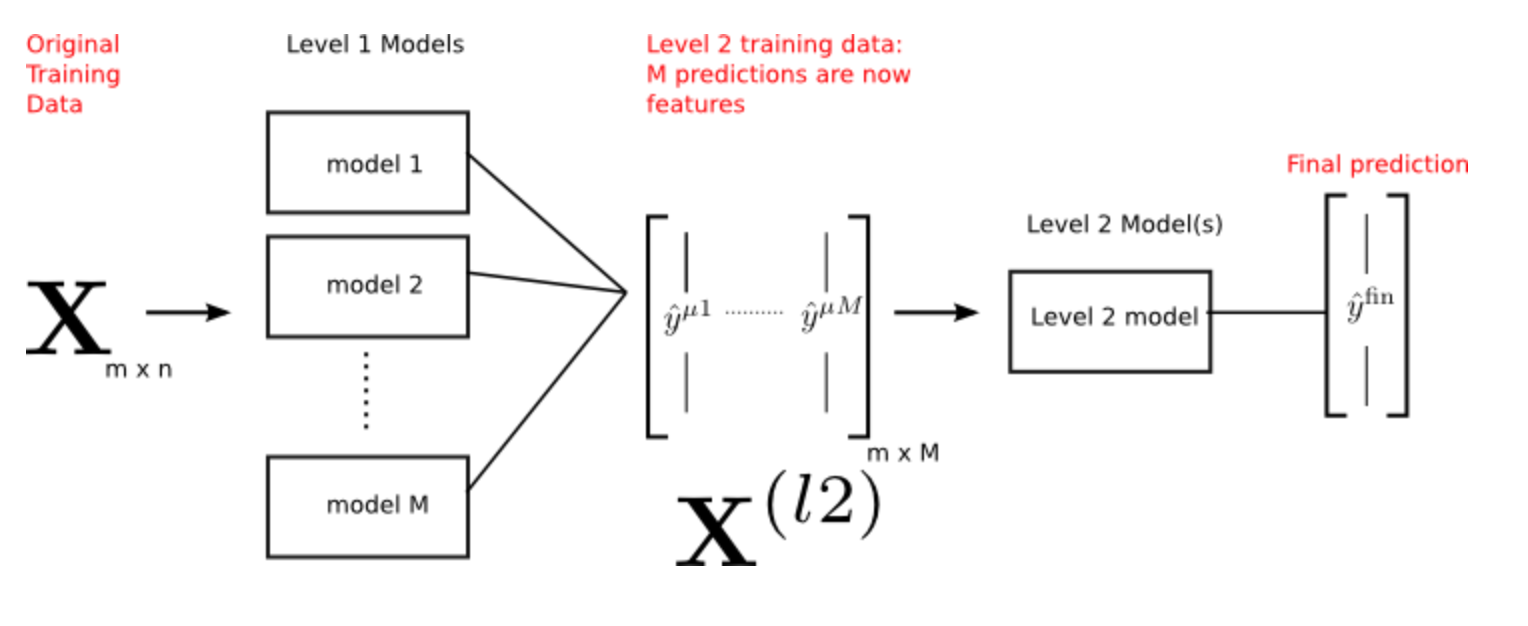
\includegraphics[width=0.8\textwidth]{stack_model}
        \caption{Diagram of the stack model, it illustrates the format of input data for second layer classifier in the stacked model. Diagram borrowed from \cite{stack2017}.}
        \label{stack}
        \end{figure}
    \end{itemize}

    \item \boldline{Details of models and techniques} \\
        We optimized \textbf{first layer models} in isolation, using CV to choose the best model parameters, details below:
        \begin{itemize}
            \item \textbf{K Nearest Neighbors:} trained KNN for a wide range of $N \in \{2^i | i \in [1,10]\}$ with three different distance metrics for each $N$: Manhattan, Euclidean, and Bray-Curtis to explore how these different metrics work with our sparse/high-dimensional dataset.
            \item \textbf{AdaBoost:} with parameter search across the number of estimators and the learning rate. For most experiments we set the learning rate to 1. There is a trade-off between the learning rate for Adaboost and the number of estimators or weak classifiers. The learning rate reduces the contribution of each classifier by this learning rate. Hence we decide on learning rate first, then we search for the best number of estimators.
            \item \textbf{Random Forest:} with parameter search across the max depth and minimum split size, with number of estimators first set at 10 for the random search, then set at 250 for the grid search.
            \item \textbf{Extra Trees:} with parameter search across number of estimators. Note that Extra Trees (extremely randomized trees) can be used only as ensemble model because they work just like Random Forest but here the cut-point is selected at random.
            \item \textbf{XGBoost:} with randomized parameter search across maximum tree depth, learning rate, subsample ratio of columns when constructing each tree, subsample ratio of the training instance and minimum loss reduction required to make a further partition on a leaf node of the tree - gamma. Followed by manual parameter tuning according to training/validation loss curves.
            \item \textbf{Logistic Regression:} with parameter search across regularization constant $C$ and maximum number of iterations
            \item \textbf{FFM:} We used libFFM's implementation of field-aware factorization machines \cite{juan2016field}. FFMs have been shown to be effective in the classification of sparse data.
            \item \textbf{Neural Nets:} We experimented with different network architectures, we used bagging and dropout to prevent overfitting. We also incorporated to the first layer models a neural network with input data from other word representations including:
                \begin{itemize}
                    \item Word embeddings: we used fasttext implementation with pretrained word vectors for our embeddings, then we classified the embeddings using a convolutional neural network with batch normalization and dropout to prevent overfitting.
                \end{itemize}
                For all our neural networks we used cross entropy loss and ADAM optimizer for gradient updates.
        \end{itemize}

        For \textbf{second layer models}, we experimented with:
        \begin{itemize}
            \item \textbf{Neural Net:} with varying size of hidden layer and varying probability dropout layers. In the end, by using one of the simpler neural nets we tried with fewer inputs from first-level models, this is what was used to achieve our best performance on the public dataset.
            \item \textbf{Logistic Regression:} used as a very simple second-layer model to serve as a baseline for model simplicity in our work to reduce overfitting.
            \item \textbf{AdaBoost w/ ExtraTrees:}
                This model was actually the best individual performing on the private dataset, but we did not use it as it had poorer performance on the public dataset.
            \item \textbf{XGBoost:} This model turned out to perform worse than the other models on the validation set and we did not use it.

        \end{itemize}

\end{itemize}

\subsection{Scrapped approaches}
We initially experimented a lot with neural nets, since they were giving the most promising results and were suited for handling high dimensionality of the data, while also easy to regularize with a array of techniques at our disposal (Dropout, batch norm, L1/L2, shared weights). For the longest time, they were our best performing models before we tried stacking.

Automated machine learning pipelines using genetic programming (AutoML)\cite{Olson2016EvoBio}! This one was a fun experiment, although we found that it did not work well compared to manual model selection and took way too long to justify it's performance.

We've also heavily experimented with XGBoost \cite{chen2016xgboost}, after all it's claim to fame is that half of all kaggle competitions are won using it, see figures \ref{xg}, \ref{xgover}, \ref{xgunder}.


\section{Model Selection}
\medskip
\begin{itemize}

    \item \boldline{Scoring} \\
    Cross validation and holdout validation are both used for scoring of models without submitting to the scoreboard. We found both approaches to be an effective (5 or 3 fold CV and 25\% holdout) estimate of actual model performance. It is suggested\cite{citeulike:13776474} that holdout validation of a respectable size is as effective and faster than cross-validation.

    Due to the 0-1 loss metric (or accuracy) not being a smooth function, surrogate loss functions are used for many of out models, like Area-under-Curve for XGBoost and logloss for Vowpal Wabbit.

    We present below the accuracies we achieved for the first layer classifiers of the stacked model and parameters that achieved them. We decided to present accuracies only for types classifiers that we used in our final model.

    \begin{itemize}
    \item \textbf{K Nearest Neighbors}
    \begin{table}[H]
\centering
\caption{KNN validation errors with different $k$ values and different parameter metrics}
\label{knn}
\begin{tabular}{l|l|l|l|}
\cline{2-4}
                               & Manhattan distance & Euclidean distance & Bray - Curtis distance \\ \hline
\multicolumn{1}{|l|}{$k=2$} & 0.6335 & 0.6128 & 0.7086 \\ \hline
\multicolumn{1}{|l|}{$k=4$} & 0.6558 & 0.6318 & 0.7357 \\ \hline
\multicolumn{1}{|l|}{$k=8$} & 0.6724 & 0.6425 & 0.7586 \\ \hline
\multicolumn{1}{|l|}{$k=16$} & 0.6842 & 0.6643 & 0.7767 \\ \hline
\multicolumn{1}{|l|}{$k=32$} & 0.6861 & 0.6787 & 0.7863 \\ \hline
\multicolumn{1}{|l|}{$k=64$} & 0.6838 & 0.6746 & 0.7904 \\ \hline
\multicolumn{1}{|l|}{$k=128$} & 0.6659 & 0.6388 & 0.7913 \\ \hline
\multicolumn{1}{|l|}{$k=256$} & 0.6315 & 0.5945 & 0.7916 \\ \hline
\multicolumn{1}{|l|}{$k=512$} & 0.5873 & 0.5455 & 0.7876 \\ \hline
\multicolumn{1}{|l|}{$k=1024$} & 0.5487 & 0.5147 & 0.7853 \\ \hline

\end{tabular}
\end{table}

So we found that the Bray-Curtis distance performed best and specifically selected the $k=128$ model with Bray-Curtis as a balance of performance and model simplicity.
\item \textbf{Extra Trees}: Here we performed a random parameter search followed by a simple grid search over the number of estimators. We used Gini criterion and we had no maximum tree depth. 200 estimators turned out to give us the best result of 0.842389 validation accuracy.
\item \textbf{Logistic Regression}: Here we performed a parameter search over the maximum number of iterations and the regularization constant. Our two best models achieved accuracy of 0.8459 with parameters $max_iter = 500$ and $C=1$ and the accuracy of 0.8466 with parameters max_iter $= 500$ and $C=0.5$.
    \item \textbf{AdaBoost:} Adaboost with parameter grid search over number of estimators, based on previous results from randomized search, learning rate set to 1. \\
    \begin{table}[H]
\label{adaboost}
\begin{minipage}[t]{.48\linewidth}
\caption{Number of estimators incremented \\ by 10, starting with 200}
      \centering
\begin{tabular}{|l|l|}
\hline
Number of estimators & Validation accuracy \\ \hline
200                  & 0.82975             \\ \hline
210                  & 0.8303              \\ \hline
220                  & 0.8299              \\ \hline
230                  & 0.82985             \\ \hline
240                  & 0.83145             \\ \hline
250                  & 0.83115             \\ \hline
260                  & 0.83235             \\ \hline
270                  & 0.8335              \\ \hline
280                  & 0.8346              \\ \hline
290                  & 0.83495             \\ \hline
300                  & 0.83415             \\ \hline
310                  & 0.83365             \\ \hline
320                  & 0.83385             \\ \hline
330                  & 0.8339              \\ \hline
340                  & 0.83365             \\ \hline
350                  & 0.83415             \\ \hline
360                  & 0.83425             \\ \hline
370                  & 0.83545             \\ \hline
380                  & 0.83495             \\ \hline
390                  & 0.83425             \\ \hline
\end{tabular}
\end{minipage}%
\begin{minipage}[t]{.48\linewidth}
\caption{Number of estimators incremented by 1, starting with 370 which gave the best accuracy for intervals of 10.}
\begin{tabular}{|l|l|}
\hline
Number of estimators & Validation accuracy \\ \hline
371                  & 0.83555             \\ \hline
372                  & 0.8353              \\ \hline
373                  & 0.8356              \\ \hline
374                  & 0.8356              \\ \hline
\end{tabular}
\begin{figure}[H]
                \centering
                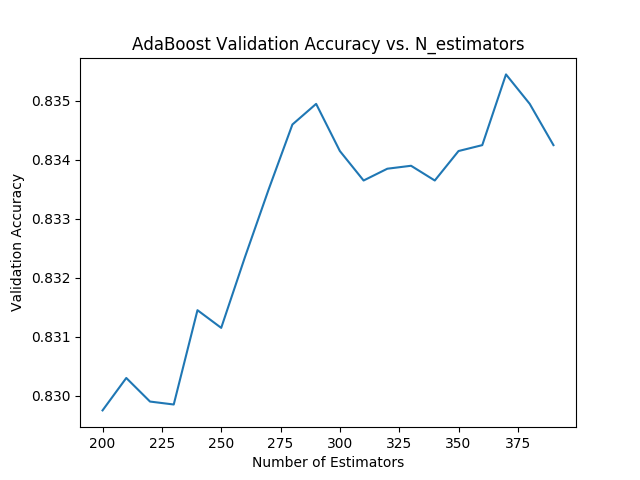
\includegraphics[width=\textwidth]{adaboost_validation_accuracy.png}
                \caption{AdaBoost training and validation accuracy vs. number of estimators.}
                \end{figure}
\end{minipage}%
\end{table}

    Hence we found the best performing model to be the one with number of estimators set to 373 or 374. We also used the model with 290 estimators because it also achieved high accuracy and it differs significantly from the best model.
    \item \textbf{Random Forest:} Random Forest with parameter grid search over maximum tree depth and the minimum number of samples required to split internal node. Grid search was based on previous results from randomized search, number of estimators for the grid search was set to 250. \\
    \begin{table}[H]
    \centering
    \caption{Table on the left presents the grid search over maximum tree depth with two different minimum numbers of samples required to split internal node i.e. 80 and 100. The middle table presents the grid search over maximum tree depth with minimum numbers of samples required to split internal node set to 80. Table to the right shows the results of the grid search over minimum numbers of samples required to split internal node, with the maximum tree depth set to 144, which performed best in the search with fixes minimum samples split.}
\label{rf}
\begin{minipage}[t]{.33\textwidth}
\begin{tabular}{l|l|l|}
\cline{2-3}
                                & $l=80$  & $l=100$ \\ \hline
\multicolumn{1}{|l|}{$d = 120$} & 0.8285  & 0.82865 \\ \hline
\multicolumn{1}{|l|}{$d=122$}   & 0.8276  & 0.8279  \\ \hline
\multicolumn{1}{|l|}{$d=124$}   & 0.8266  & 0.828   \\ \hline
\multicolumn{1}{|l|}{$d=126$}   & 0.82665 & 0.82885 \\ \hline
\multicolumn{1}{|l|}{$d=128$}   & 0.8298  & 0.82745 \\ \hline
\end{tabular}
\end{minipage}%
\begin{minipage}[t]{.33\textwidth}
\begin{tabular}{|l|l|}
\hline
Maximum     & Validation  \\
tree depth  & accuracy \\ \hline
$d=130$            & 0.82855             \\ \hline
$d=132$            & 0.82985             \\ \hline
$d=134$            & 0.8296              \\ \hline
$d=136$            & 0.8279              \\ \hline
$d=138$            & 0.82785             \\ \hline
$d=140$            & 0.82925             \\ \hline
$d=142$            & 0.82815             \\ \hline
$d=144$            & 0.83135             \\ \hline
$d=145$            & 0.82845             \\ \hline
\end{tabular}
\end{minipage}%
\begin{minipage}[t]{.33\textwidth}
\begin{tabular}{|l|l|}
\hline
Minimum     & Validation  \\
split       & accuracy \\ \hline
$l=81$            & 0.82965             \\ \hline
$l=83$            & 0.82715             \\ \hline
$l=85$            & 0.82805              \\ \hline
$l=87$            & 0.8305              \\ \hline
$l=89$            & 0.828             \\ \hline
\end{tabular}
\end{minipage}
\end{table}
We decided to use two Random Forest models in the first layer of the final stacked model. The first one with parameters: max tree depth = 132 and minimum sample split = 80, the second one with parameters: max tree depth = 144 and minimum sample split = 80. Both models use 250 estimators.
    \item \textbf{XGBoost}: We performed a randomized parameter search across many parameters (maximum tree depth, learning rate, subsample ratio of columns when constructing each tree, subsample ratio of the training instance and minimum loss reduction required to make a further partition on a leaf node of the tree - gamma). It was then followed by the parameter tuning based on the learning curves, see figures \ref{xg}, \ref{xgover}, \ref{xgunder}.
    Below we present some of the learning curves.
    \begin{figure}[H]
    \centering
    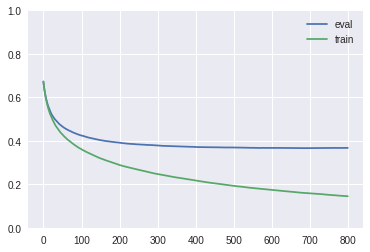
\includegraphics[width=0.5\textwidth]{xgboost}
    \caption{A sample learning curve for XGBoost parameter tuning, x-axis represents the number of iterations and y-axis represents the log-loss. Green curve is the validation loss and blue is the training loss.}
    \label{xg}
    \end{figure}
    \begin{minipage}{0.43\textwidth}
    \begin{figure}[H]
    \centering
    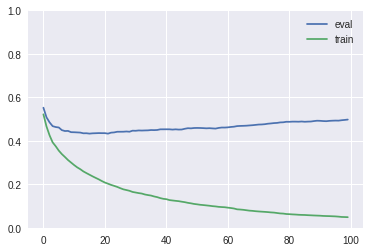
\includegraphics[width=\textwidth]{xg_over}
    \caption{A learning curve for XGBoost parameter tuning, shows overfitting example, x-axis represents the number of iterations and y-axis represents the log-loss. Green curve is the validation loss and blue is the training loss.}
    \label{xgover}
    \end{figure}
    \end{minipage}\hfill
    \begin{minipage}{0.43\textwidth}
    \begin{figure}[H]
    \centering
    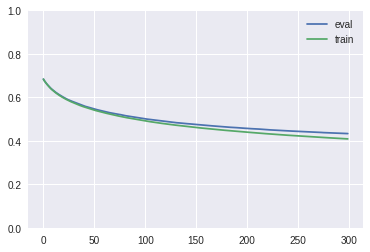
\includegraphics[width=\textwidth]{xg_under}
    \caption{A learning curve for XGBoost parameter tuning, shows underfitting example, x-axis represents the number of iterations and y-axis represents the log-loss. Green curve is the validation loss and blue is the training loss.}
    \label{xgunder}
    \end{figure}
    \end{minipage}
    \item \textbf{Neural Nets}: We ended up using two neural networks in the first layer of our stacked model. We tried using the convolutional neural network with the words embeddings as inputs but it turned out to perform worse than the neural networks that were using the bag-of-words model. We experimented with different network architectures, the two that gave us best validation accuracy are:
    \begin{itemize}
    \item Validation accuracy: 0.8569; 10 Bags of Input 1000 (Dropout 0.2) $\rightarrow$ Dense 128 ReLU, L2 regularizer $\lambda = 0.001$ (Dropout 0.5) $\rightarrow$ Dense 2, Softmax
    \item Validation accuracy: 0.8502; 10 Bags of Input 1000 $\rightarrow$ Dense 256 ReLU, L2 regularizer $\lambda = 0.01$ (Dropout 0.5) $\rightarrow$ Dense 128 ReLU, L2 regularizer $\lambda = 0.01$ (Dropout 0.5) $\rightarrow$ Dense 64 ReLU, L2 regularizer $\lambda = 0.01$ (Dropout 0.5) $\rightarrow$ Dense 32 ReLU, L2 regularizer $\lambda = 0.01$ (Dropout 0.5) $\rightarrow$ Dense 2, Softmax
    \end{itemize}
    For all our neural networks we used categorical cross entropy loss and ADAM optimizer for gradient updates.
    \end{itemize}

    \item \boldline{Validation and Test} \\

    In the table below we present the scores from public and private leaderboard of our most successful submissions.

    \begin{table}[H]
\centering
\caption{Our final results for different models.}
\label{results}
\begin{tabular}{l|l|l|}
\cline{2-3}
                                                                                                                                    & Public leaderboard & Private Leaderboard \\ \hline
\multicolumn{1}{|l|}{\begin{tabular}[c]{@{}l@{}}2-layer stacked model with\\ logistic regression in 2nd layer\end{tabular}}         & 0.85460            & 0.85700             \\ \hline
\multicolumn{1}{|l|}{\begin{tabular}[c]{@{}l@{}}2-layer stacked model with\\ neural network in 2nd layer\\ and dropout reduced to 25\%\end{tabular}}              & 0.85740            & 0.85780             \\ \hline
\multicolumn{1}{|l|}{\begin{tabular}[c]{@{}l@{}}2-layer stacked model with\\ neural network in 2nd layer\end{tabular}}              & 0.86060            & 0.85960             \\ \hline
\multicolumn{1}{|l|}{3-layer stacked model (*)}                                                                                     & 0.85500            & 0.85440             \\ \hline
\multicolumn{1}{|l|}{\begin{tabular}[c]{@{}l@{}}2-layer stacked model with\\ AdaBoost with Extra Trees\\ in 2nd layer\end{tabular}} & 0.85600            & 0.86080             \\ \hline
\end{tabular}
\end{table}
All models presented here used the first-layer individual models described in detail in the previous section (Scoring).\\
(*) the 3-layer stacked model details:
\begin{itemize}
\item 1st layer: same 2-layer stacked models
\item 2nd layer: Random Forest, Gradient Boosting Forest and Neural Network classifiers
\item 3rd layer: Random Forest classifier
\end{itemize}

In our final set of submissions, we used a limited set of first-layer individual models based on their first-layer validation accuracy:
\begin{itemize}
\item KNN with $k=128$ and Bray-Curtis distance.
\item AdaBoost models with $n_\textrm{est} \in \{290,373\}$
\item Random Forest models with $d_\textrm{max} \in \{132,144\}$ and min split size of 80
\item Extra Trees as described above
\item Two neural nets trained on the bag of words model as described above.
\end{itemize}

\begin{figure}[h!]
\centering
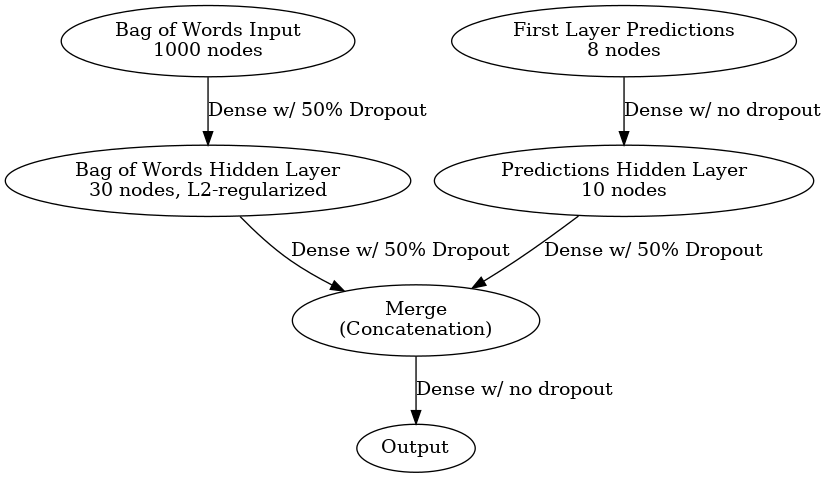
\includegraphics[width=0.8\textwidth]{final_nn.png}
\caption{Final neural net model which achieved the best score on public leaderboard: used in a classifier with four bags; all nodes with ReLU activation except the output with softmax.}
\end{figure}


\end{itemize}

\section{Conclusion}
\medskip
\begin{itemize}

    \item \boldline{Discoveries} \\
        One major discovery was that overfitting became problematic very quickly. Our approach of stacking results from many distinct models using a second-layer model which itself (in most forms we explored) contained many different parameters allowed us to achieve validation accuracies close to 0.9, but these models would only achieve 0.84-0.85 accuracies on the test dataset. We posited that this overfitting came from some combination of:
        \begin{itemize}
        \item Overfitting in the first-layer models themselves.
        \item Utilizing too many distinct first-layer models in the stacked model, allowing it too much expressiveness in second-layer training.
        \item Complexity of the second-layer model, for which at first we were using neural nets with 40-50 nodes in a hidden layer, and AdaBoost with Extra Trees.
        \item Data leakage from first-layer cross-validation predictions used as training inputs in the second-layer training.
        \end{itemize}
        While we explored all of these possibilities to some extent, the most fruitful step we took was in decreasing the number of submodel inputs to the stacked model. Our best performing stacked model on the public leaderboard was a neural net with 40 hidden nodes, but with only 8 sets of first-layer model predictions rather than as much as 45 that we had been using previously. By selecting the eight models with the best validation accuracy in the first layer and throwing out the rest entirely, our validation accuracy for the stacked model decreased around 2-3\%, but the test accuracy increased by 0.5-1\%!

        On the other hand, attempts to reduce overfitting by using simpler first-layer models and drastically decreasing the complexity of our second-layer model by trying logistic regression ultimately failed, resulting in models that performed worse as measured by both validation accuracy and test accuracy on the leaderboard.

        Another surprising discovery was the futility of data transformations to intuitively more ``expressive'' forms such as TF-IDF and embeddings. Our suspicion is that the increased dimensionality resulting from using embeddings rather than the 1000-words bag-of-words was a major culprit for this approach's ineffectiveness -- perhaps by performing some dimensionality reduction this approach could still have merit. Intuitively, semantic representations should provide extra external information about the positive/negative sentiment of words among many other things -- if we could reduce the amount of information in these representations to dimensions more relevant to sentiment, we may start to see positive results.

    \item \boldline{Challenges} \\
        One challenge we consistently faced is the difficulty of parameter tuning for so many models. Fortunately, we were able to get reasonable results faster by using a randomized parameter search instead of grid search. However, when we wanted to analyze in-sample vs. out-of-sample performance across a wide range of parameter values, we found it time-consuming to generate the plots needed to make these calls on whether we should choose simpler models in order to minimize overfitting.

        At one point, we attempted to address the potential data leaking problem noted in ``Discoveries'' by training our first layer models on a subset of the training data and maintaining a 10\% holdout. However, we found ourselves having to make a number of practical compromises -- it would have been too time-consuming to reoptimize the parameters for all of our models from scratch, so for the most part we used parameters learned from cross-validation on all of the data and just retrained the model on the smaller subset of data using those parameters, which is of course a case of data leakage itself. Additionally, this created a new practical concern throughout our code to ensure that the dimensions stayed consistent and vectors of cardinality 18000 didn't mix with those of 20000. In the end, these complications prevented us from exploring the effects of data leakage from one stage of the stacked model to the next as much as we would have liked to.

        Finally, we tried using keras models as base estimators in AdaBoost, but it was not supported. We added support for it in a \href{https://github.com/keras-team/keras/pull/9252}{PR}.


    \item \boldline{Concluding Remarks} \\
        Our final model benefited from many of the discoveries and learnings discussed above, and we were able to achieve much better results with a stacked model than with any single first-layer model. We were then able to achieve even better results when we simplified our stacked model to decrease the impact of overfitting.

        However, there are a number of loose threads we were unable to explore to the depth we would have liked to, and we know that we could likely achieve much better results were we to further explore more expressive representations like embeddings as well as find a better balance of simplicity and expressiveness in our second-layer model.

\end{itemize}

\bibliography{mp1}
\bibliographystyle{ieeetr}


\end{document}
